\documentclass{article}
\usepackage[margin=3pt,landscape]{geometry}
\usepackage{tikz}
\usepackage{amsmath}
\usepackage{svg}
\usepackage{xcolor}
\usepackage[cache=false]{minted}
\usepackage{pdflscape}
\usepackage{longtable}
\usepackage{array}
\usepackage{adjustbox}


\usetikzlibrary {arrows.meta,bending,positioning} 

\usetikzlibrary{shapes.geometric, shapes.arrows}
\usetikzlibrary{patterns}
\usetikzlibrary{quantikz2}
     \tikzset{operator/.append style={fill=white!0}}


\newsavebox{\incode} 
\newsavebox{\fmovecode}
\newsavebox{\fmoveqiskit}
\newsavebox{\smovecode}
\newsavebox{\smoveqiskit}
\newsavebox{\ffcapturecode}
\newsavebox{\ffcaptureqiskit}
\newsavebox{\fhcapturecode}
\newsavebox{\fhcaptureqiskit}
\newsavebox{\mcode}
\newsavebox{\mqiskit}


\begin{document}

% Save tabular in a box
\savebox{\fmovecode}{%
    \begin{tabular}[t]{l}
        board[i] = \textcolor{blue}{None} \\ 
        board[i+d1, i+d2] = \{\\
            \quad \textcolor{orange}{'color'} : \textcolor{blue}{red}, \\
            \quad \textcolor{orange}{'probability'} : \textcolor{blue}{0.5}, \\
            \quad \textcolor{orange}{'pawn'} : \textcolor{blue}{1}\} \\
    \end{tabular}
}

\savebox{\incode}{%
\begin{tabular}[t]{l} 
    board[i] = \{\\ 
        \quad \textcolor{orange}{'color'} : \textcolor{blue}{red}, \\ 
        \quad \textcolor{orange}{'probability'} : \textcolor{blue}{1}, \\ 
        \quad \textcolor{orange}{'pawn'} : \textcolor{blue}{1} 
        \} 
    \end{tabular}
}

\savebox{\fmoveqiskit}{%
    \begin{tabular}[t]{l} 
        circuit.ch(q[i], q[i+d1]) \\
        circuit.swap(q[i], q[i+d2]) \\
        circuit.cx(q[i+d1], q[i+d2])
    \end{tabular}
}

\savebox{\smovecode}{%
    \begin{tabular}[t]{l}
        board[i, j] = \textcolor{blue}{None} \\ 
        board[$i+d_{1,2}, j+d_{1,2}$]\\
        = \{\textcolor{orange}{'color'} : \textcolor{blue}{red}, \\
            \quad \textcolor{orange}{'probability'} : \textcolor{blue}{0.25}, \\
            \quad \textcolor{orange}{'pawn'} : \textcolor{blue}{1}\} \\
    \end{tabular}
}

\savebox{\smoveqiskit}{%
\begin{tabular}[t]{l} 
    circuit.ch(q[i], q[i+d1]) \\
    circuit.ch(q[j], q[j+d1]) \\
    circuit.swap(q[i], q[i+d2]) \\
    circuit.swap(q[j], q[j+d2]) \\
    circuit.cx(q[i+d1], q[i+d2]) \\
    circuit.cx(q[j+d1], q[j+d2])
\end{tabular}
}

\savebox{\ffcapturecode}{%
    \begin{tabular}[t]{l}
        board[i] = \textcolor{blue}{None} \\ 
        board[i+d1, i+d2+1] = \{\\
            \quad \textcolor{orange}{'color'} : \textcolor{blue}{red}, \\
            \quad \textcolor{orange}{'probability'} : $\mathcolor{blue}{(1/2)}$, \\
            \quad \textcolor{orange}{'pawn'} : \textcolor{blue}{1}\} \\
    \end{tabular}
}

\savebox{\ffcaptureqiskit}{%
\begin{tabular}[t]{l} 
    circuit.ch(q[i], q[i+d1]) \\
    circuit.swap(q[i], q[i+d2]) \\
    circuit.cx(q[i+d1], q[i+d2]) \\
    circuit.cx(q[i+d2+1], q[i+d2])
\end{tabular}
}

\savebox{\fhcapturecode}{%
    \begin{tabular}[t]{l}
        board[i, j] = \textcolor{blue}{None} \\ 
        board[$i+d_{12}, j+d_1$,\\
            \quad $j+d_1+1$] = \{\\
            \quad \textcolor{orange}{'color'} : \textcolor{blue}{red}, \\
            \quad \textcolor{orange}{'probability'} : $\mathcolor{blue}{1/4}$, \\
            \quad \textcolor{orange}{'pawn'} : \textcolor{blue}{1}\} \\
    \end{tabular}
}

\savebox{\fhcaptureqiskit}{%
\begin{tabular}[t]{l} 
    circuit.ch(q[i], q[i+d1]) \\
    circuit.swap(q[i], q[i+d2]) \\
    circuit.cx(q[i+d1], q[i+d2]) \\
    circuit.cx(q[i+d2+1], q[i+d2])
\end{tabular}
}


\savebox{\mcode}{%
    \begin{tabular}[t]{l}
        for i in range(0,c.len()):\\
            \quad if c[i] == 0:\\
            \quad\quad board[i] = None\\
            \quad else:\\
            \quad\quad board[i]['probability'] = 1\\
    \end{tabular}
}

\savebox{\mqiskit}{%
\begin{tabular}[t]{l} 
    for ($q_i,c_i$) in zip(q,c): \\
    \quad circuit.measure($q_i,c_i$)
\end{tabular}
}

        \begin{center}
            \begin{longtable}[t]{||p{5em} p{15em} p{8em} p{29em} p{14em}||} 
            \hline
            Move name & Move & Python list & Quantum array & Qiskit \\ [0.5ex] 
            \hline\hline
            \raggedright \adjustbox{valign=b}{Initialize} & \adjustbox{valign=b}{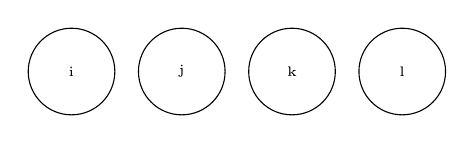
\begin{tikzpicture}
    \def\d{1.4}
    \def\size{1.1}
    \node(c1) [circle, draw, minimum size = \size cm] at (\d * 0,0) {\tiny i};
    \node(c2) [circle, draw, minimum size = \size cm] at (\d * 1,0) {\tiny j};
    \node(c3) [circle, draw, minimum size = \size cm] at (\d * 2,0) {\tiny k};
    \node(c4) [circle, draw, minimum size = \size cm] at (\d * 3,0) {\tiny l};
\end{tikzpicture}} & \adjustbox{valign=b}{$\text{board=[\textcolor{blue}{None}] * 32}$} & \adjustbox{valign=b}{\begin{quantikz}[scale=1.5]
   \lstick{${\ket{0}_i}$} & \\
   \lstick{${\ket{0}_j}$}  &\\
   \lstick{${\ket{0}_k}$}  &\\
   \lstick{${\ket{0}_l}$} &
\end{quantikz}} &  \adjustbox{valign=b}{\begin{tabular}{l} q = QuantumRegister(10, \textcolor{orange}{'q'}) \\ circuit = QuantumCircuit(q)\end{tabular}} \\ [1ex]
            \hline
            \adjustbox{valign=b}{New pawn} & \adjustbox{valign=b}{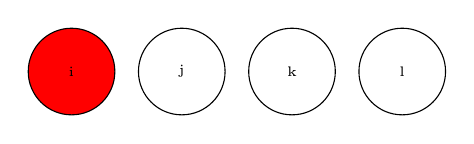
\begin{tikzpicture}
    \def\d{1.4}
    \def\size{1.1}
    \node(c1) [circle, draw, fill=red, minimum size = \size cm] at (\d * 0,0) {\tiny i};
    \node(c2) [circle, draw, minimum size = \size cm] at (\d * 1,0) {\tiny j};
    \node(c3) [circle, draw, minimum size = \size cm] at (\d * 2,0) {\tiny k};
    \node(c4) [circle, draw, minimum size = \size cm] at (\d * 3,0) {\tiny l};
\end{tikzpicture}} & \adjustbox{valign=b}{\usebox{\incode}} & \adjustbox{valign=b}{\begin{quantikz}[scale=1.5]
    \lstick{$\ket{0}_i$} & \gate{X} & \rstick{$\ket{1}_i$}\\
    \lstick{$\ket{0}_j$}& &\\
    \lstick{$\ket{0}_k$} &&\\
    \lstick{$\ket{0}_l$} &&\\[-1em]
\end{quantikz}} & \adjustbox{valign=b}{circuit.x[q[i]]} \\
            \hline
            \adjustbox{valign=b}{First move} & \adjustbox{valign=b}{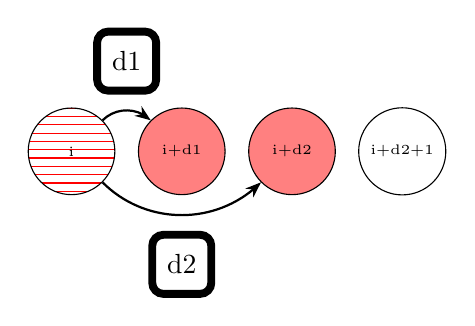
\begin{tikzpicture}
    \def\d{1.4}
    \def\size{1.1}
    \node(c1) [circle, draw, minimum size = \size cm, pattern={horizontal lines},pattern color=red] at (\d * 0,0) {\tiny i};
    \node(c2) [circle, draw, minimum size = \size cm, fill = red!50] at (\d * 1,0) {\tiny i+d1};
    \node(c3) [circle, draw, minimum size = \size cm, fill = red!50] at (\d * 2,0) {\tiny i+d2};
    \node(c4) [circle, draw, minimum size = \size cm] at (\d * 3,0) {\tiny i+d2+1};

    \draw[draw, thick, -{Stealth[length=2mm]}]
    (c1) edge [bend left=45] node[pos=0.5, above, rectangle, draw, minimum width = 0.75 cm, minimum height = 0.75 cm, rounded corners, line width = 0.1 cm, yshift=0.2cm] {d1} (c2)
    (c1) edge [bend right=45] node[pos=0.5, below, rectangle, draw, minimum width = 0.75 cm, minimum height = 0.75 cm, rounded corners, line width = 0.1 cm, yshift=-0.2cm] {d2} (c3);
\end{tikzpicture}} & \adjustbox{valign=b}{\usebox{\fmovecode}} & \adjustbox{valign=b}{\begin{quantikz}[color=gray, scale=1]
    \lstick{\small$i\;$} & \setwiretype{q} & \ctrl{1} & \ctrl{2} & \gate{X}& \\
    \lstick{\small$i+d1\;$} & \setwiretype{q} & \targ{ } &          & \gate{H}& \\
    \lstick{\small$i+d2\;$} & \setwiretype{q} &          & \targ{ } & \gate{H}& 
\end{quantikz}} & \adjustbox{valign=b}{\usebox{\fmoveqiskit}} \\
            \hline
            \adjustbox{valign=b}{Second move} & \adjustbox{valign=b}{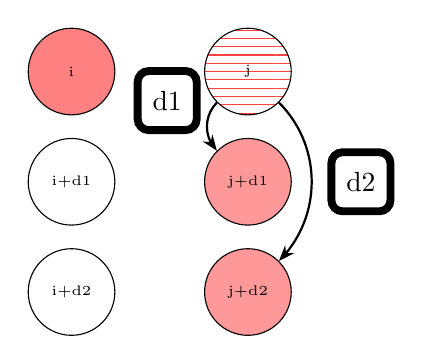
\begin{tikzpicture}
    \def\d{1.4}
    \def\w{1.6}
    \def\size{1.1}
    \node(c1) [circle, draw, minimum size = \size cm, fill=red!50] at (\d * 0,0) {\tiny i};
    \node(c2) [circle, draw, minimum size = \size cm, pattern={horizontal lines},pattern color=red!75] at (\d * \w,0) {\tiny j};
    \node(c3) [circle, draw, minimum size = \size cm] at (\d * 0,-\d *1) {\tiny i+d1};
    \node(c4) [circle, draw, minimum size = \size cm] at (\d * 0,-\d*2) {\tiny i+d2};
    \node(c5) [circle, draw, minimum size = \size cm, fill = red!40] at (\d * \w,-\d*1) {\tiny j+d1};
    \node(c6) [circle, draw, minimum size = \size cm, fill = red!40] at (\d * \w, -\d * 2) {\tiny j+d2};


    \draw[draw, thick, -{Stealth[length=2mm]}]
    (c2) edge [bend right=45] node[pos=0.3, left, rectangle, draw, minimum width = 0.75 cm, minimum height = 0.75 cm, rounded corners, line width = 0.1 cm, xshift=-0.1cm, yshift=0.2cm] {d1} (c5)
    (c2) edge [bend left=45] node[pos=0.5, right, rectangle, draw, minimum width = 0.75 cm, minimum height = 0.75 cm, rounded corners, line width = 0.1 cm, xshift=0.2cm] {d2} (c6);

\end{tikzpicture}}& \adjustbox{valign=b}{\usebox{\smovecode}} & \adjustbox{valign=b}{\begin{quantikz}[scale=1]
    \lstick[wires=2]{$\ket{10}_{ij}+\ket{01}_{ij}$}        & \ctrl{2} & \ctrl{4} & \swap{3}     &              &            & \rstick{\ket{0}}\\
                                                           &          &          &              & \swap{4}     &            & \rstick{\ket{0}}\\
    \lstick{$\ket{0}_{i+d_1}$}                             & \gate{H} &          &              &              & \ctrl{1}   & \rstick[wires=4]{\begin{tabular}[t]{l} \ket{1000} \\ +\ket{0100} \\ +\ket{0010} \\ +\ket{0001} \end{tabular}}\\
    \lstick{$\ket{0}_{i+d_2}$}                             &          &          & \swap{-3}    &              & \targ{-1}  &                 \\
    \lstick{$\ket{0}_{j+d_1}$}                             &          & \gate{H} &              &              & \ctrl{1}   &                 \\
    \lstick{$\ket{0}_{j+d_2}$}                             &          &          &              & \swap{-4}    & \targ{-1}  &
\end{quantikz}} & \adjustbox{valign=b}{\usebox{\smoveqiskit}} \\
            \hline
            \adjustbox{valign=b}{full-full capture} & \adjustbox{valign=b}{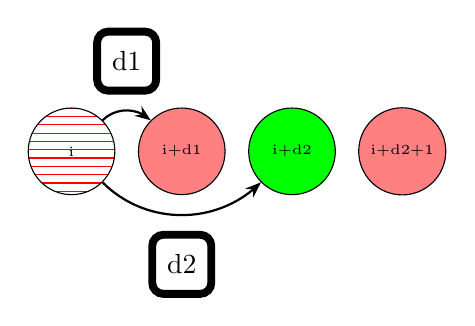
\begin{tikzpicture}
    \def\d{1.4}
    \def\size{1.1}
    \node(c1) [circle, draw, minimum size = \size cm, pattern={horizontal lines},pattern color=red] at (\d * 0,0) {\tiny i};
    \node(c2) [circle, draw, minimum size = \size cm, fill = red!50] at (\d * 1,0) {\tiny i+d1};
    \node(c3) [circle, draw, minimum size = \size cm, fill = green] at (\d * 2,0) {\tiny i+d2};
    \node(c4) [circle, draw, minimum size = \size cm, fill =red!50] at (\d * 3,0) {\tiny i+d2+1};

    \draw[draw, thick, -{Stealth[length=2mm]}]
    (c1) edge [bend left=45] node[pos=0.5, above, rectangle, draw, minimum width = 0.75 cm, minimum height = 0.75 cm, rounded corners, line width = 0.1 cm, yshift=0.2cm] {d1} (c2)
    (c1) edge [bend right=45] node[pos=0.5, below, rectangle, draw, minimum width = 0.75 cm, minimum height = 0.75 cm, rounded corners, line width = 0.1 cm, yshift=-0.2cm] {d2} (c3);
\end{tikzpicture}} & \adjustbox{valign=b}{\usebox{\ffcapturecode}} &\adjustbox{valign=b}{\begin{quantikz}[color=gray, scale=1]
    \lstick{\small$i\;$} & \setwiretype{q} & \ctrl{1} & \ctrl{2} & \gate{X}& \\
    \lstick{\small$i+d1\;$} & \setwiretype{q} & \targ{ } &          & \gate{H}& \\
    \lstick{\small$i+d2\;$} & \setwiretype{q} &          & \targ{ } & \gate{H}& 
\end{quantikz}} & \adjustbox{valign=b}{\usebox{\ffcaptureqiskit}} \\
            \hline
            \adjustbox{valign=b}{1 half-half capture} & \adjustbox{valign=b}{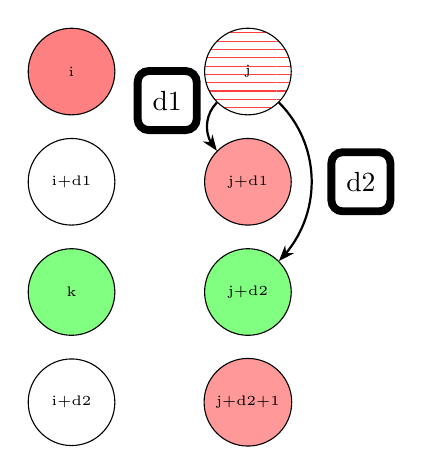
\begin{tikzpicture}
    \def\d{1.4}
    \def\w{1.6}
    \def\size{1.1}
    \node(c1) [circle, draw, minimum size = \size cm, fill=red!50] at (\d * 0,0) {\tiny i};
    \node(c2) [circle, draw, minimum size = \size cm, pattern={horizontal lines},pattern color=red!75] at (\d * \w,0) {\tiny j};
    \node(c3) [circle, draw, minimum size = \size cm] at (\d * 0,-\d *1) {\tiny i+d1};
    \node(c4) [circle, draw, minimum size = \size cm, fill = green!50] at (\d * 0,-\d *2) {\tiny k};
    \node(c5) [circle, draw, minimum size = \size cm] at (\d * 0,-\d*3) {\tiny i+d2};
    \node(c6) [circle, draw, minimum size = \size cm, fill = red!40] at (\d * \w,-\d*1) {\tiny j+d1};
    \node(c7) [circle, draw, minimum size = \size cm, fill = green!50] at (\d * \w, -\d * 2) {\tiny j+d2};
    \node(c8) [circle, draw, minimum size = \size cm, fill = red!40] at (\d * \w, -\d * 3) {\tiny j+d2+1};



    \draw[draw, thick, -{Stealth[length=2mm]}]
    (c2) edge [bend right=45] node[pos=0.3, left, rectangle, draw, minimum width = 0.75 cm, minimum height = 0.75 cm, rounded corners, line width = 0.1 cm, xshift=-0.1cm, yshift=0.2cm] {d1} (c6)
    (c2) edge [bend left=45] node[pos=0.5, right, rectangle, draw, minimum width = 0.75 cm, minimum height = 0.75 cm, rounded corners, line width = 0.1 cm, xshift=0.2cm] {d2} (c7);

\end{tikzpicture}} & \adjustbox{valign=b}{\usebox{\fhcapturecode}} &\adjustbox{valign=b}{\begin{quantikz}[scale=1]
    \lstick[wires=2]{$\ket{10}_{ij}+\ket{01}_{ij}$}        &  &     &           &\rstick[wires=4]{\begin{tabular}[t]{l} $\sqrt{2}$\ket{1000}\\ + \ket{0001}\\ + \ket{0010}  \end{tabular}}\\
                                                           & \ctrl{1} & \swap{2}  &           & \\
    \lstick{$\ket{0}_{j+d_1}$}                             & \gate{H} &             & \ctrl{1}  & \\
    \lstick{$\ket{0}_{j+d_2}$}                             &          & \swap{-2}   & \targ{-1} &
\end{quantikz}} & \adjustbox{valign=b}{\usebox{\fhcaptureqiskit}} \\
            \hline
            \adjustbox{valign=b}{Measure}           &                                                   & \adjustbox{valign=b}{\usebox{\mcode}} & \adjustbox{valign=b}{\begin{quantikz}[scale=1.5]
    \setwiretype{n} & & & \lstick{$\psi_i$} & \setwiretype{q} & \meter{}&\\
    \setwiretype{n} & & & \lstick{$\psi_j$} & \setwiretype{q} & \meter{}&\\
    \setwiretype{n} & & & \lstick{$\psi_k$} & \setwiretype{q} & \meter{}&\\
\end{quantikz}} & \adjustbox{valign=b}{\usebox{\mqiskit}} \\
            \hline
            \end{longtable}
        \end{center}

\end{document}
